\chapter{Forbidden C++ Forward Indirect Calls Exposed}
\label{C++ Bad Forward Indirect Calls}

\section{Polymorphism in C++}
\label{Late Binding in C++}
Polymorphism along inheritance and encapsulation
are the most used modern object-oriented concepts
in C++. 
Polymorphism in C++ allows to access different types of objects 
through a common base class. A pointer of the type of the base object
can be used to point to object(s) which are derived from the base class.
In C++ there is:
\textit{a)} compile-time (or static, usually is implemented with templates), 
\textit{b)} run-time (dynamic, is implemented with inheritance and virtual functions), 
\textit{c)} ad-hoc polymorphism (e.g., if the range of actual types that can be used 
is finite and the combinations must be individually specified prior to use), and
\textit{d)} parametric polymorphism (e.g., if code is written without mention of any 
specific type and thus can be used transparently with any number of new types it
is called parametric polymorphism). 
The first two are implemented through early 
and late binding, respectively.
In C++, overloading concepts fall under the category of \textit{c)} and Virtual functions;
templates or parametric classes fall under the category of pure polymorphism.
C++ provides polymorphism through: 
\textit{i)} virtual functions,
\textit{ii)} function name overloading, and 
\textit{iii)} operator overloading. 
In this paper, we will be concerned with dynamic 
polymorphism---based on virtual functions (10.3 and 11.5 in 
ISO/IEC N3690~\cite{iso:iecN3690})---because these can be exploited to 
call: illegitimate vtables in the class hierarchy 
or fake vtables.
Virtual functions have several uses and issues associated, 
but for the scope of this paper will look at the indirect 
call sites which are generated when objects are invoking these type
of functions. More precisely, 
\textit{1)} load-time enforcement: as calling each indirect call site (callee) requires 
a fix number of parameters which are passed each time the caller is calling, we
enforce a fine-grained CFI policy by statically determining the number and types of all function parameter
that belong to an indirect call site.
\textit{2)} run-time verification: as checking during run-time legitimate from
illegitimate indirect caller/callee pairs requires parameter type (along parameter number),
we check during run-rime before each indirect call-site if the caller matches to the callee 
based on the previously added checks.


allows an object of one type to access



Explain how late binding is implemented in C++ and which role virtual functions play.
How is late binding basically implemented.

There is compile time Polymorphism and there is run time polymorphism.
Compile time polymorphism is realized through early binding and run time
polymorphism is realized through late binding.


\newsavebox{\firstlisting}
\begin{lrbox}{\firstlisting}
\begin{minipage}[c]{0.48\textwidth}
\begin{minted}[
% frame=lines,
framesep=2mm,
linenos,
frame=none,
firstnumber=1,
framesep = 1.0cm,
% baselinestretch=1.2,
% bgcolor=LightGray,
fontsize=\footnotesize,
]{C++}
class nsMultiplexInputStream final 
 :public nsIMultiplexInputStream 
 ,public nsISeekableStream //B1
 ,public nsIIPCSerializableInputStream //B2
 ,public nsICloneableInputStream{ //B3
nsTArray<nsCOMPtr<nsIInputStream>> mStreams;
NS_IMETHODIMP nsMultiplexInputStream::Close(){
  MutexAutoLock lock(mLock);
  mStatus = NS_BASE_STREAM_CLOSED;
  //set NS_OK flag
  nsresult rv = NS_OK;
  //get array length
  uint32_t len = mStreams.Length();
  //array-based main loop gadget
 for (uint32_t i = 0; i<len; ++i){
  //(1) hijacked indirect call
  nsresult rv2=mStreams[i]->Close();
  if (NS_FAILED(rv2)) {
      rv = rv2;
  }
 }
  return rv;
}
\end{minted}
\end{minipage}
\end{lrbox}

\begin{figure}
 \begin{minipage}{.48\textwidth}
\usebox{\firstlisting}
\end{minipage}%%
\hfill
%&
%
\hspace{2.2cm}
\begin{minipage}{.48\textwidth}
    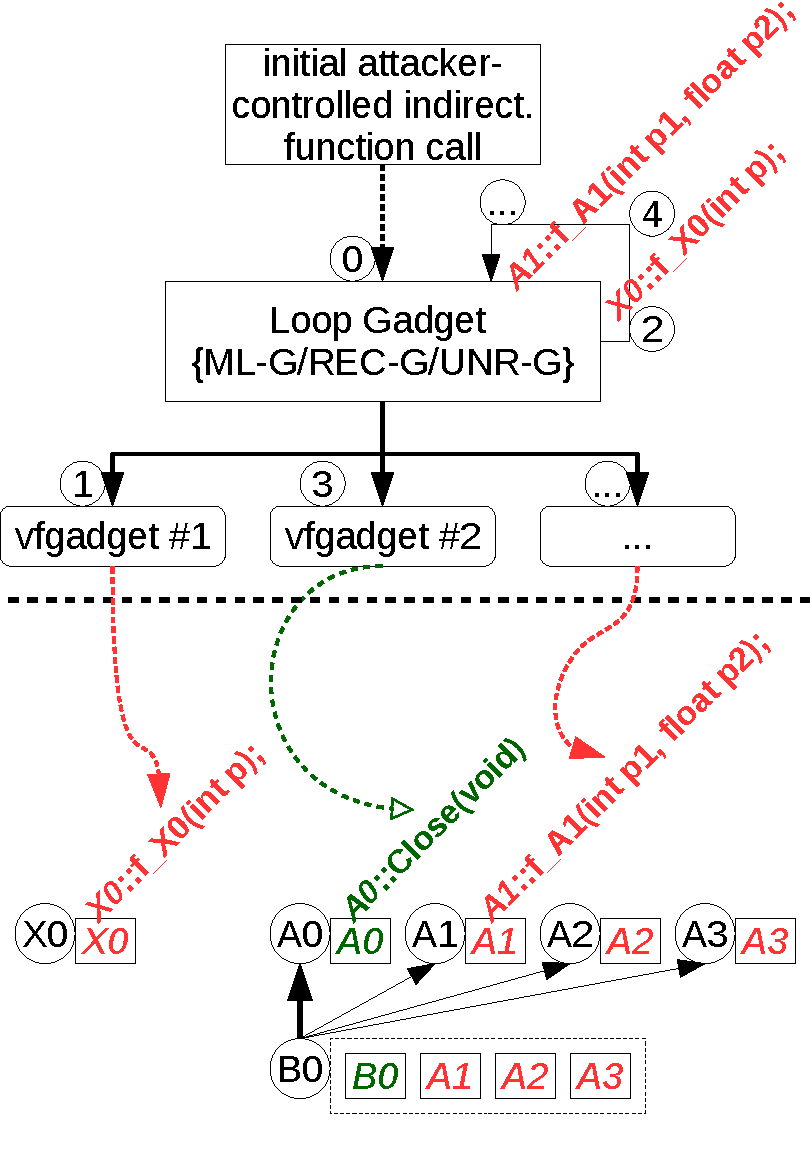
\includegraphics[width=0.95\textwidth]{figures/loop.pdf}
\end{minipage}
\caption{bla}
\end{figure}

%%second pic
\begin{figure}
    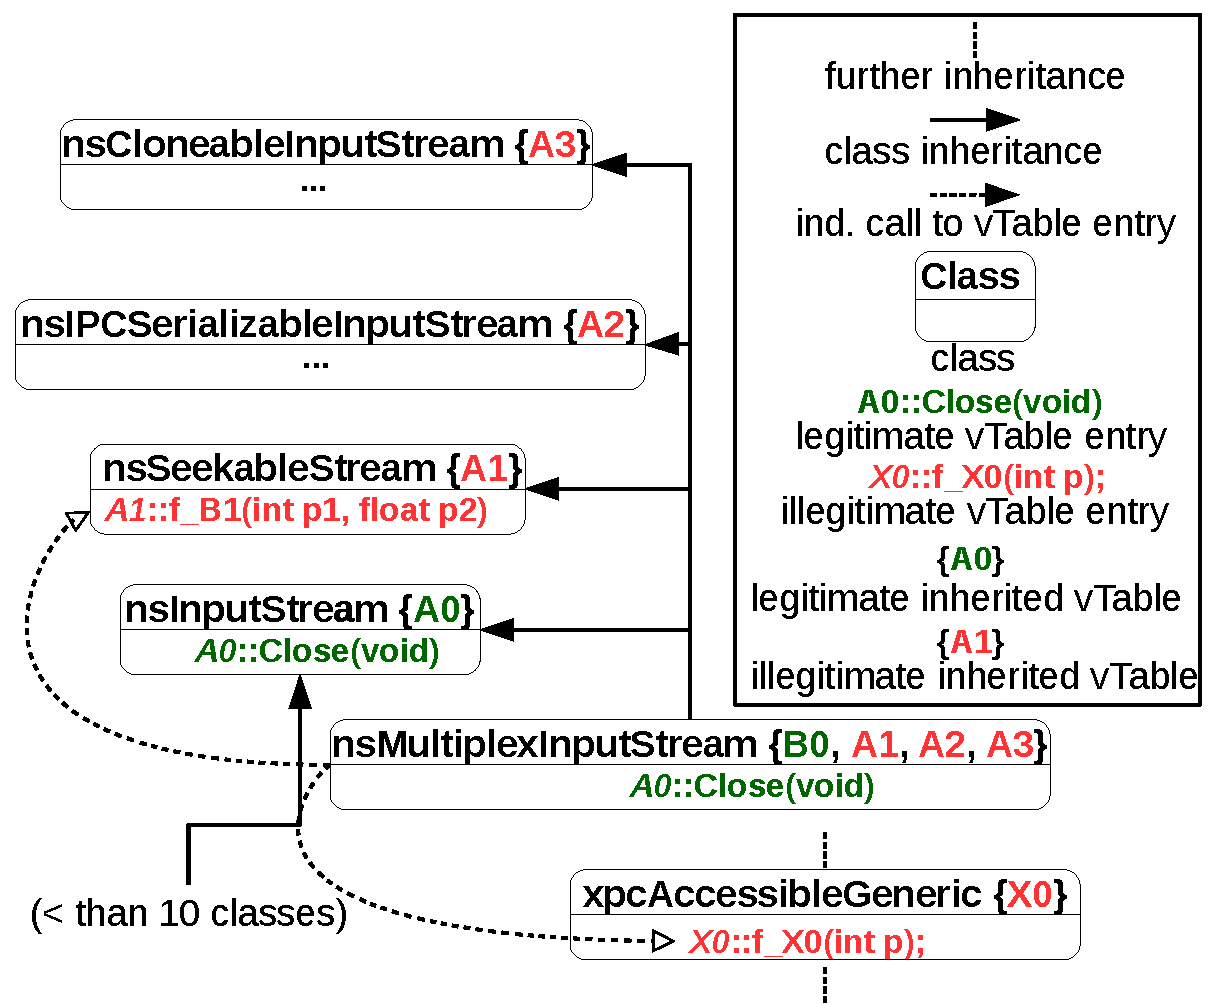
\includegraphics[width=0.7\textwidth]{figures/class_hierarchy.pdf}
\caption{bla 2}
\end{figure}

\section{Virtual Dispatch in Practice}
\label{Virtual Dispatch in Practice}

\section{Security Implications of Forbidden C++ Forward Indirect Calls}
\label{Security Implications of Virtual Dispatch}

How can Forbidden C++ Forward Indirect Calls exploited?
First through COOP attacks,
vptr corruption and then fake vtable insertion an reuse
or reuse of avaialble v tables.

Second, the available vtables in a large class hierarchy can represent 
another attack surface since a sufficiently large class hierarchy can provide
many useful gadgets for an attacker.

\section{Running Example: CVE X}
\label{Running Example: CVE X}
CVE-2014-3176


show the class hierarchy of the classes involved in the exploit.
Draw also the associated v tables along the classes.







